\documentclass[11pt]{article}
\usepackage[letterpaper, margin=0.8in]{geometry}
\usepackage{amsmath}
\usepackage{amssymb}
\usepackage{wrapfig}
\usepackage[makeroom]{cancel}
\usepackage{bbm}
\usepackage{booktabs}
\usepackage{float}
\usepackage{array}
\usepackage{bm}
\usepackage{enumerate}
\usepackage{amsfonts} 
\usepackage{color}
\usepackage{hyperref}
\usepackage{xcolor}
\usepackage{hyperref}
\usepackage{newfloat}
\usepackage{graphicx}
\usepackage{caption}
\usepackage{fancyhdr}
\usepackage{bbm}
\usepackage[overload]{empheq}
\newcommand{\IF}{\text{if }}
\def\changemargin#1#2{\list{}{\rightmargin#2\leftmargin#1}\item[]}
\let\endchangemargin=\endlist 
\newcommand{\norm}[1]{\left\lVert#1\right\rVert}

\title{Copy Number Change Point Analysis with Cell-Specific Shifts}

\begin{document}
\maketitle
\section{Introduction}

\section{Method}
\subsection{Model}
\noindent We model the copy number data for probe $i$ of sample $j$ like the following. $Y_{ij}$ is the data we observe for sample $j$'s probe $i$, and $\Theta_{ij}$ is the underlying true copy number for probe $i$ in sample $j$. $\phi$ is a probe-effect while $\xi$ is a cell-specific shifts which is the main attribution of this package. 
\begin{equation}
Y_{ij} = (\Theta_{ij}+\xi_j)\phi_i + \epsilon_{ij}, \text{  } \epsilon_{ij} \sim N(0, \sigma^2)
\end{equation}

\noindent In order to find make recover the piece-wise constant $\Theta$, we solve the following penalized regression equation under the assumption that if there are change points in copy number, it is likely to be shared among the samples. 

\begin{equation}
min_{\phi, \xi, \Theta} \sum_{i,j} (Y_{ij} - \xi_j \phi_i -  \Theta_{ij} \phi_i)^2 + \sum_{i=1}^p \lambda \frac{\|\Theta_{i+1\cdot} - \Theta_{i\cdot}  \|}{w_i}
\end{equation}

\subsection{Alternating Descent}
We use an alternating descent algorithm to update $\Theta$, $\phi$, and $\xi$ \cite{wang2016estimating}. 
\begin{itemize}
\item
\textbf{Update $\Theta$ given ($\phi$ and $\xi$) through Group Fused Lars \cite{bleakley2011group}}\\
If we substitute $Y_{ij}$ to $Y_{ij} - \xi_j \phi_i$ for all $i$ and $j$, the Group Fused Lars algorithm is the same with the method from Wang, Chen, \& Zhao (2016) \cite{wang2016estimating}
$$\Theta = argmin_{\Theta} \sum_{i,j} ((Y_{ij} - \xi_j \phi_i) - \phi_i \Theta_{ij})^2 + \sum_{i=1}^{p} \lambda \frac{\|\Theta_{i+1\cdot} - \Theta_{i\cdot}  \|}{w_i} $$

\item
\textbf{Update $\phi$  given ($\xi$ and $\Theta$) by solving least squares}\\
For all probe $i$, we can solve the least squares problem and get a closed-form update for $\phi_i$. 
$$argmin_{\phi_i} \sum_{i,j}(Y_{ij} - (\Theta_{ij}+\xi_j)\phi_i)^2$$
$$ =  \frac{\sum_j (\Theta_{ij} + \xi_j)Y_{ij}}{
\sum_j (\Theta_{ij}+\xi_j)^2
}$$
\item
\textbf{Update $\xi$ given ($\phi$ and $\Theta$) by solving least squares}\\
Similarly, we can get a closed form update for $\xi$.
$$argmin_{\xi_j} \sum_{i,j} (Y_{ij} - \phi_i \Theta_{ij} - \phi_i \xi_j)^2$$
$$= \frac{
\sum_i (Y_{ij}-\phi_i \Theta_{ij})\phi_i
}{
\sum_i \phi_i^2
}$$
\end{itemize}

\subsection{Constraints for identifiability}
\noindent We limit the L2 norm of $\phi$ to the length of the vector $\phi$, and we constrain the mean of $\xi$ to be 0. An interpretation of this constraint is like that of random effects centered at zero. We don't however impose any distributional assumption.

\noindent Also, in order to prevent the sign-flipping due to the probe effect $\phi$, at the last step of the algorithm, we multiplied the sign of $\phi$ to the resulting $\Theta$ values in order to match the sign of $Y$ value. For example, when $Y$ is positive for certain sample, it is possible that since $\phi$ is negative, 

\section{Data}
We tested our method with three public data sets. First data set labeled as `encode' is from K562 cell lines from the ENCODE project whose bulk sequencing data is available as well, enabling the verification of the result. The second and third ones come from Ginkgo's web tool for analyzing single-cell sequencing data. We took polygenomic breast tumor data and circulating lung tumor cells where each of them were sequenced through DOP-PCR and MALBAC respectively. \\

\noindent Ginkgo provides the normalized read counts data. For the analysis of copy number, we took the log ratio of the read counts over 2. When the read counts for sample $j$ on probe $i$ 

\section{Results}
\noindent We ran the algorithms assuming two models below for multiple data sets to compare their performances. The older model without the cell-specific effects is labeled "MBAmethyl" as the original package name, and the new method is labeled "cnvJoint" as our new package name. 

\begin{align*}
\text{MBAmethyl : }&Y_{ij} = \Theta_{ij} * \phi_i + \epsilon_{ij}\\
\text{cnvJoint : }&Y_{ij} = (\Theta_{ij} + \xi_j)*\phi_i + \epsilon_{ij}
\end{align*}

\noindent Our main focus lies on the difference between the $\Theta$s from the two models. Specifically, we compare the heterogeneity of $\Theta$ within and across the clusters. We assume that samples $j$ within the same cluster, $\Theta_{ij}$ should be very close to one another - for example, normal cells should have log ratio of copy numbers at 0 for all $i$. Across clusters, we believe it is better to have higher distance measure so that it is easy to differentiate tumor types. \\


\noindent For the Ginkgo data sets, we normalized the copy numbers in the following way. First of all, we discovered the 'normal cells' through clustering. Then for each of those samples, we removed the outliers by taking 25\% and 75\% quantile for each sample $j$. Then we took the median for each $j$. Then we took the mean of those medians across all the samples, and took that as our baseline copy number for each probe. So we divided every element by the baseline and took $log$. Therefore, for normal cells, we expect constant log ratio 0 for all probes, but we expect either positive or negative shifts in tumor cells. We do not expect all tumors to have the same copy number variation pattern, but we expect the change point will tend to be shared across the tumor cells within the same cluster.\\

The euclidean distance between two cells was normalized by the number of probes : 
$$\Lambda_{i,j} = \sum_{l=1}^{p} (\Theta_{l, i} - \Theta_{l, j})^2 / p$$
$\Lambda$ is visualized in Figure \ref{diffmat}.


\begin{figure}[h]
\centering
\includegraphics[width=0.49\textwidth]{encode_MBAmethyl_theta_heat.pdf}
\includegraphics[width=0.49\textwidth]{encode_cnvJoint_theta_heat.pdf}\\
\includegraphics[width=0.49\textwidth]{poly_MBAmethyl_theta_heat.pdf}
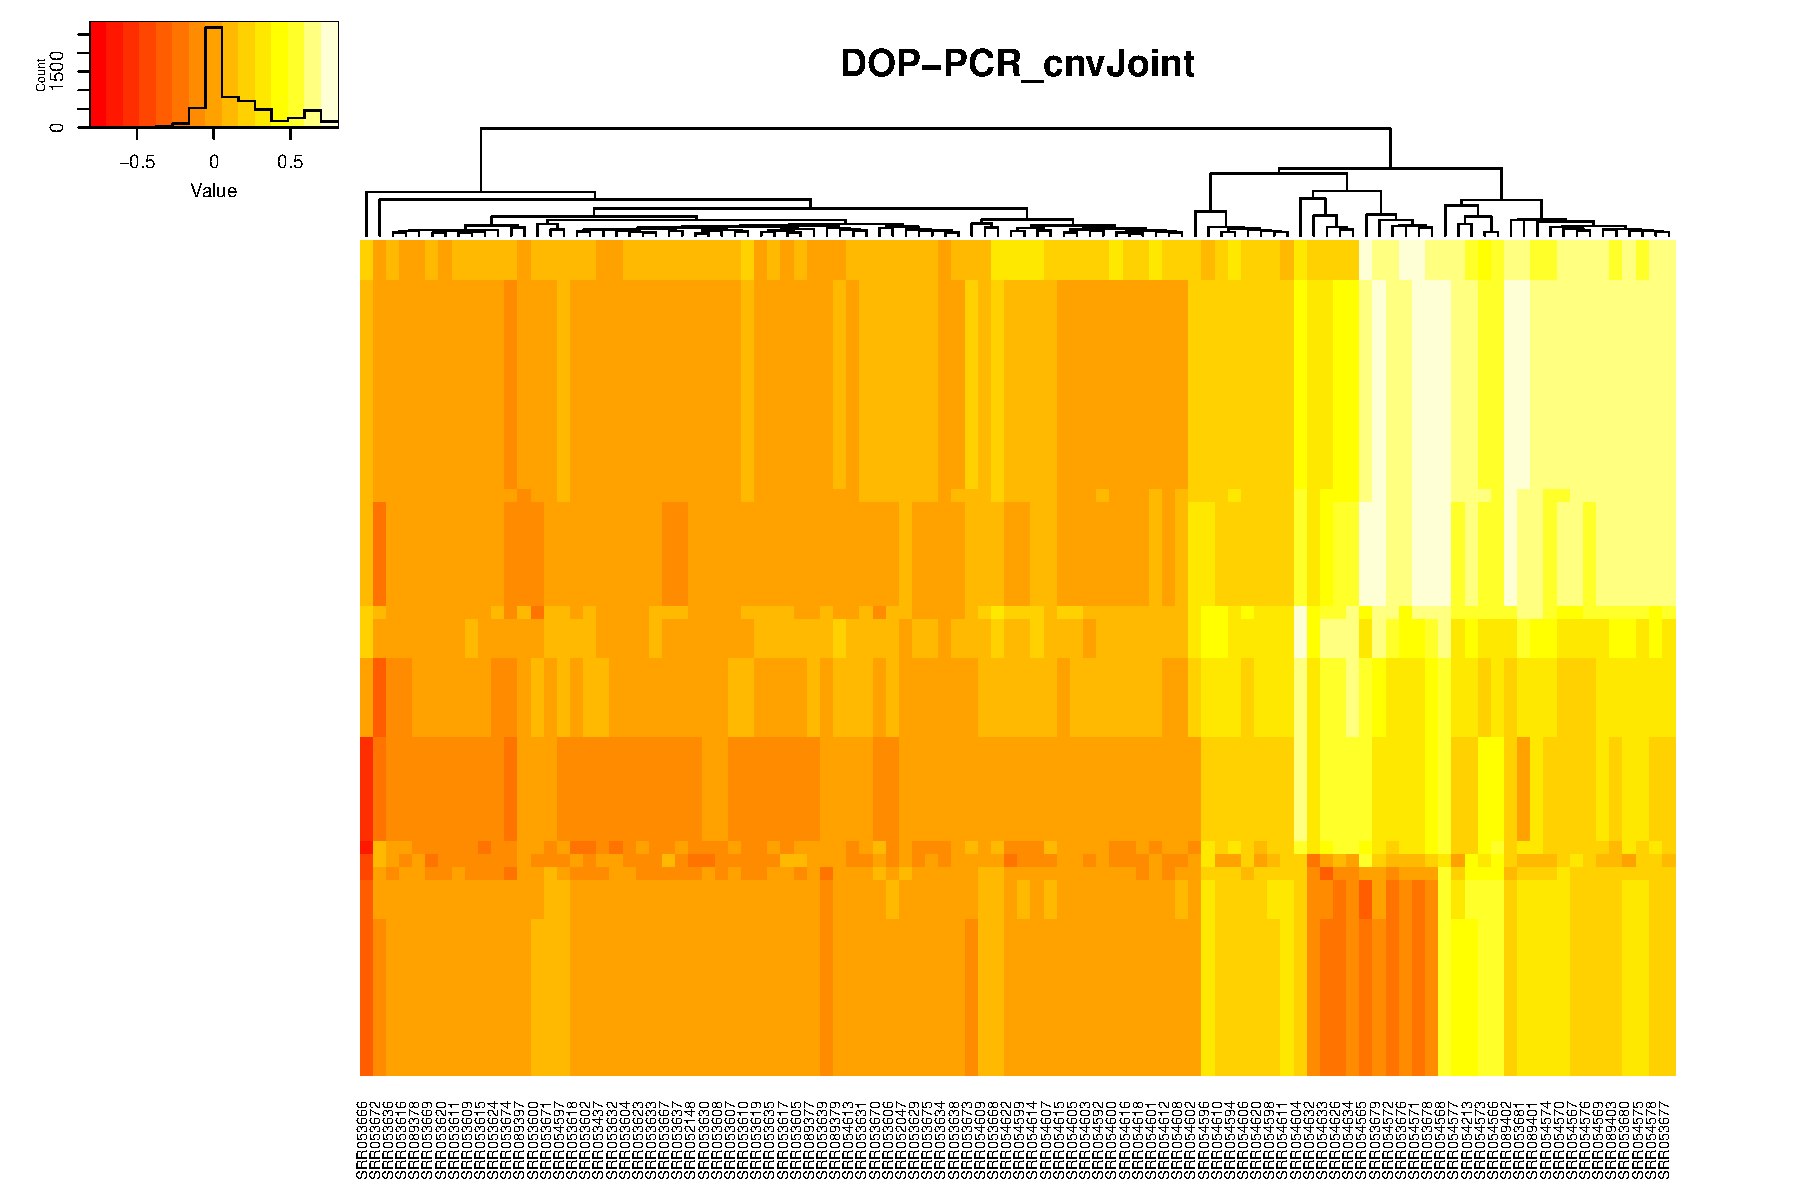
\includegraphics[width=0.49\textwidth]{poly_cnvJoint_theta_heat.pdf}\\
\includegraphics[width=0.49\textwidth]{lung_MBAmethyl_theta_heat.pdf}
\includegraphics[width=0.49\textwidth]{lung_cnvJoint_theta_heat.pdf}
\caption{\label{thetaheatmap}
\textbf{Comparison of heatmap for $\Theta$ from cnvJoint and MBAmethyl}
}
\end{figure}

\begin{figure}[h]
\centering
\includegraphics[width=0.8\textwidth]{encode_distmat_heat.pdf}\\
\includegraphics[width=0.8\textwidth]{poly_distmat_heat.pdf}\\
\includegraphics[width=0.8\textwidth]{lung_distmat_heat.pdf}\\
\caption{\label{distmat_heat}
\textbf{Comparison of distance matrix for $\Theta$}\\
The cell-cell euclidean distance in terms of copy numbers is computed for the three data sets. The clusters are determined by hierarchical clustering using euclidean distance. 
}
\end{figure}

\begin{figure}[h]
\centering
\includegraphics[width=0.45\textwidth]{intraclusters_bar.pdf}
\includegraphics[width=0.45\textwidth]{acrossclusters_bar.pdf}\\
\caption{\label{diff_bar}
\textbf{Difference in intra-cluster and cross-cluster distance}\\
The bar graph shows that in most cases, average intra-cluster distance is smaller for cnvJoint, suggesting more homogeneity is returned by our new approach. In contrast, when average distance is computed across different clusters, e.g. between normal cells versus tumor cells, cnvJoint returned higher average distance for most cases, suggesting clearer distinction between the cell types. 
}
\end{figure}

\begin{figure}[h]
\centering
\includegraphics[width=0.8\textwidth]{dist_xi.png}
\caption{\label{dist_xi}
\textbf{Distribution of $\xi$}\\The values of $\xi$ values for the three data types. This essentially measures the effectiveness of our new method compared to MBAmethyl. Due to the nature of the data, the individual shifts have small effects on Ginkgo data sets that have been sufficiently cleaned. 
}
\end{figure}



\bibliographystyle{plain}
\bibliography{cite}


\end{document}







